\subparagraph{Predication Example 1: }
Consider the following code sequence.

\begin{verbatim}

00	r2 <- r1 op r0
10	b_op r2, 030
20	r3 <- r1 op r0
30	r4 <- r1 op r0

\end{verbatim}

This example illustrates a simple minimal control dependency
situation.
Instruction 30 does not depend, either through a data flow dependency
or a control flow dependency, on any of the instructions that
are shown to be before it.  The branch instruction 10 is data
dependent on instruction 00 (through register
{\tt r2}.
Instruction 20 is control
dependent on instruction 10 (the branch).
The branch is initially predicted to be not-taken.
The execution sequence of this example is shown
in Figure
Figure~\ref{pex1}.

\begin{figure}
\centering
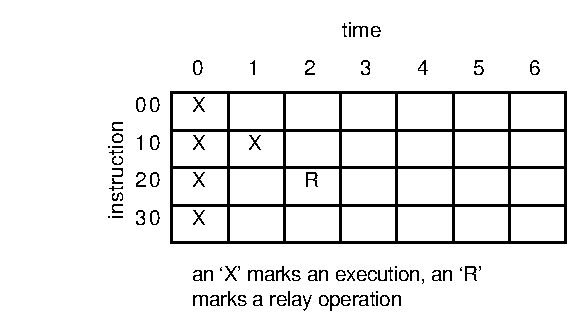
\epsfig{file=pex1.eps,height=1.50in}
\caption{{\em Timing of the code example, predication scenario 1.}
This example illustrates the exploitation of basic minimal control
dependencies, a significant contribution to
achieving higher ILP by taking advantage of independent
instructions beyond the joins of branches.
Execution of an instruction at a given time is
again indicated by an `X'.}
\label{pex1}
\end{figure}

We start by assuming that all instructions execute in a single clock
cycle and that they all execute immediately upon being loaded.
It is assumed that the initial execution of the branch in
instruction 10 (at time 0) did not change its predicate output.
However, since instruction 00 executed in clock cycle 0, we will
assume that its output value changed from what was originally loaded
at instruction load time.  Instruction 00 will broadcast forward
its new updated output (register
{\tt r2}).
Since instruction 10 (the branch) is data dependent on
register
{\tt r2}
from instruction 00, it will snoop for that update
and snarf the new value from the forward broadcast.  
This will enable it to re-execute.
We assume that it executes at the earliest possible time.
This would be clock cycle 1.  On this execution, its output predicate,
essentially its branch prediction, does change.  The branch may either
have been resolved at this point or simply may have made a new prediction
based on a possibly still speculative value of register
{\tt r2}.
A change in the branch condition will change its
predication output and this will be
broadcast out.
If the branch became resolved and a DEE path originating due to this
branch had been started, an implementation may abandon the
current main-line execution path and switch the DEE path of this branch
to become the new main-line path.
For this example, we will assume that
no switch to a DEE paths occurs.  When no switch to a DEE path occurs,
instruction 20, being control dependent on the branch, will be snooping
for the branch predicate change and seeing that it has changed
will switch to relaying its output value.  
The relay operation
takes the value for register
{\tt r3} that was loaded, or snarfed, from before the execution
of instruction 20, and re-broadcasts it.  The re-broadcast of the relayed 
output value is necessary in those cases where following instructions
used the previously broadcasted output value.
The relaying operation would have
also occurred
if a DEE path became the new main-line path
but implementations can choose to switch executions paths or
not as an optimization.

In spite of the branch being predicted one way and then changed
to the other (whether re-predicted or resolved), it should be
noted that instruction 30 was not required to be re-executed as
a result.  This illustrates a basic minimal control dependency
which serves to facilitate higher instruction level parallelism (ILP)
by taking advantage of independent instructions located beyond the
joins of branch domains.

\subparagraph{Predication Example 2: }
Consider the following slightly more involved example than the first.

\begin{verbatim}

00	r2 <- r0 op r1
10	b_op r2, 030
20	r2 <- r3 op r0
30	r4 <- r2 op r0

\end{verbatim}

The time ordered execution sequence for this example is shown in
Figure~\ref{pex2}.

\begin{figure}
\centering
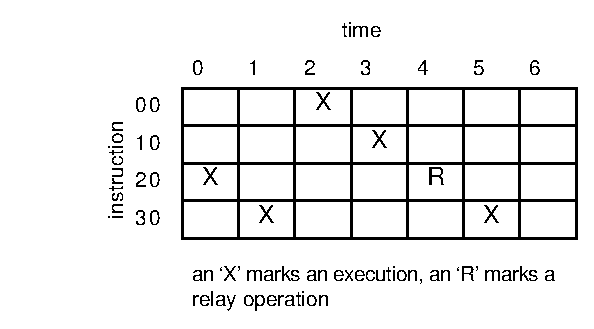
\epsfig{file=pex2.eps,width=2.50in}
\caption{{\em Timing of the code example, predication scenario 2.}
This example illustrates a relay operation that
can occur within an active station when a branch
predicate changes.
Execution of an instruction at a given time is
again indicated by an `X'.  A relay operation is indicated by an 'R'.}
\label{pex2}
\end{figure}

It is assumed that all instructions are loaded and that
the branch at 10 is initially predicted as not taken.
Since instruction 20 is not restricted from executing
due to the initial branch prediction of instruction 10,
it can execute immediately upon being loaded.
It is assumed that it does execute immediately and before
all other instruction shown.
Since instruction 30 is data dependent on instruction 20
when the branch is not taken, it snarfs up the
newly created value for register
{\tt r2}
from instruction 20 and is enabled to execute.
Instruction 30 gets to execute in the follow clock cycle.
Now, later, instruction 00 executes creating a new value for
register
{\tt r2}.
We assume that this is still a speculative value.
Note that since instruction 30 has already snarfed a value for
register
{\tt r2}
later in time than that created by instruction 00, it is not
enabled for execution due to this change.
Instruction 10, however, is data dependent on instruction 00 (through
{\tt r2})
and is enabled to execute.  
Note carefully also, that instruction 20 was snooping for both
its inputs and its output (register
{\tt r2}).  It had to snoop for newly created values for
{\tt r2}) in case it was determined that the execution the instruction
was squashed.  The new value of
register
{\tt r2} will be snarfed by instruction 20 from 
the output forward broadcast of
instruction 00.

Instruction 10, the branch now executes.
We now assume that after the branch at 10 executes, its output
predicate changes, that is, the branch is now predicted to
be taken.  Its output predicate is broadcast and
instruction 20, snooping on the branch output predicate,
sees the broadcast and snarfs it.  Instruction 20, now has
an indication that its assignment of its executed value
is no longer valid and instead broadcasts its relayed value
for register
{\tt r2}.
Finally, this newly broadcast value for
register
{\tt r2} will
be snarfed by instruction 30 enabling it to re-execute also.
Finally instruction 30 executes in clock cycle 5 as shown in the
figure above.

This example showed how the effects of instructions within the
domain of a branch are squashed when the branch either
changes to a prediction of taken or is resolved to be taken.
It also showed how the incorrect results of instructions beyond the
join of a branch are corrected when a branch outcome is changed.

\subparagraph{Predication Example 3: }
This next example illustrates a switch of a DEE path to become
the new main-line path.
Consider the following code sequence.

\begin{verbatim}

00	r2 <- r0 op r1
10	b_op r2, 030
20	r3 <- r0 op r1
30	r4 <- r0 op r1

\end{verbatim}

The time ordered execution sequence for this example is shown in
Figure~\ref{pex3}.

\begin{figure}
\centering
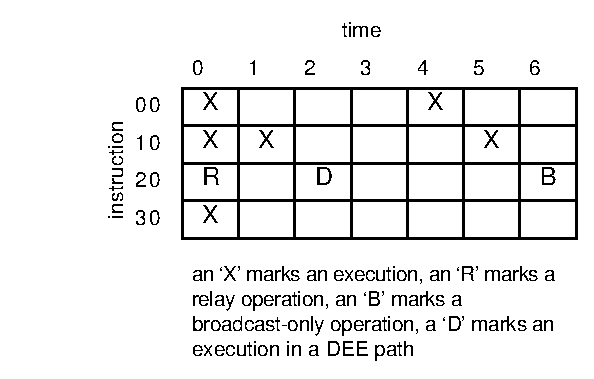
\epsfig{file=pex3.eps,width=2.50in}
\caption{{\em Timing of the code example, predication scenario 3.}
This example illustrates a switch of a DEE path to
become the new main-line path.
Execution of an instruction at a given time is
again indicated by an `X', a relay operation is indicated by an 'R',
and a broadcast-only operation is indicated by a 'B'.}
\label{pex3}
\end{figure}

It is assumed that all instructions are loaded and that
the branch at 10 is initially predicted as taken.
It is also assumed that all of the instructions are
executed immediately in main-line active stations.
Note that the execution of instruction 20 is really only
just a relay operation because it is within the domain of the branch 
in instruction 10 and the initial prediction is taken.
Because instruction 10 is data dependent on instruction 00, it
sees the newly broadcasted value
for register
{\tt r2}
from instruction 00 and becomes enabled to execute again.
It executes again in cycle 1.
This current state of execution, with regard to the instructions
shown, may persist for some time until the committed state of
the machine catches up with the current instructions.

It is now assumed that a DEE path was created, some time
after the initial executions already mentioned, and that
instruction 20 gets to execute in the DEE path.  Since
the DEE path branch output predicate is always opposite of
that of the same branch in the main-line active stations,
instruction 20 executes creating a new value for
register
{\tt r3}
rather than relaying an old value as was done with this
same instruction in the main-line path.
This newly created value for register
{\tt r3}
is broadcast and may be snarfed by following both DEE path
active stations as well as following main-line path stations.
In this example, we have not shown any future instructions
dependent on the output of instruction 20 but there could be
some instructions executing in the instruction stream after instruction 30
as shown.

Finally, at some time later again, instruction 00
re-executes, creating what will become the resolved committed
state for register
{\tt r2}.
This enabled the re-execution of instruction 10, the branch.
When the branch executes, it also finally resolves.
We will assume that the branch resolves to the no-taken
state.  This is opposite to its previous prediction, indicating
a previous misprediction, and this will cause a switch of the
DEE path to become the new main-line path.
The effect of the DEE path switch to the main-line path
causes all predicated instructions following the branch
to re-broadcast their output values.  This is seen
happening with the broadcast-only operation of
instruction 20 in cycle 6.

Although, not shown in this example, instructions in the main-line
beyond the end of the DEE path (that was switched to main-line),
will also see the effects of the branch predicate change
if they were predicated at all (either directly or indirectly)
on the output resolution of the branch of instruction 10.

